\section{Results}
\label{sec:results}

 All the tests were executed on Pianosa\footnote{Pianosa web site: \url{http://pianosa.di.unipi.it/Home_pianosa/html/info.html}}, one of the cluster of the Computer Science Department in Pisa. The cluster is composed by 24 homogeneous nodes. The nodes are 800 Mz Pentium III with 1GB of main memory and they are connected through a Fast Ethernet interconnection network. The Operating system is Fedora Core 1. On that cluster, we installed the Apache Hadoop 0.20.2 framework. The configuration parameters are set to default, so, the maximum number of task per node is set to 2 and the number of replication is set to 3. 
We decided to place the Secondary NameNode and the JobTracker in cluster interface node.
The cluster interface node is not used neither as TaskTracker nor DataNode.
21 nodes are available as slaves.

The data used in the test was generated using two matrix generators written in Matlab.
One generator for the sparse matrix A and another one for the matrices W and H. 
Both generators produce matrices containing positive elements only.
The first one is a sparse matrix generator and its sparsity factor can be tuned through an input parameter. 
The second one is dense matrix generator, the mean value of the matrix values can be selected by the user. 
For our tests, we fix the $m$ and $n$ parameters (the dimension of the A matrix) respectively to \numprint{105000} and \numprint{20000}.
All matrices value are normally distributed with a mean value of 100 and a standard deviation of 1.

For all the tests, the number of reduce task is set to $ 1,8 * number\_of\_worker$, except in the phase 3 and 4 that have 1 and 0 reducer respectively.
This choice has been driven by the Hadoop User Guide that suggest to set the reduce task number to 
$ \text{mapred.tasktracker.reduce.tasks.maximum} * number\_of\_worker * C $where C is a constant choose in the range between 0.9 and 1.8 \cite{numeroReducer}. 
The Hadoop guide claims that a value in this range should be optimal.
Specifying the number of mappers is instead quite complex since the command job.setNumMapTasks give the framework only a suggestion on the number of mappers to use.
The only way to ensure that the desired number of mappers is used is to split input files accordingly. 
Therefore, the External Phase classes (that convert the input data from text to sequence) allows the user to specify how many reducer tasks must be used. 
In that way, a corresponding number of files are produced.
Since our project is composed by five different phases executed sequentially, it is difficult to find the optimal number of Mappers and Reducers for each phase (The number of Reducers of one phase determine the number of Mappers of the next phase). 
Therefore, for testing purposes we fixed the number of reducer with respect to the number of workers.
We have chosen a value of C of 0.9, which seemed to deliver quasi optimal results for every phase.

The first set of tests shows how the computation scales in relation to the the size of the data. 
We studied how the performance change with respect to the sparsity factor of the A matrix and different k values. 
In the first test, the number of non-zero elements in the sparse matrix has been changed between \numprint{5000000} and \numprint{80000000} elements while the k parameter remains fixed to 10. 
In the second test, the k value varies between 10 and 125 while the non zero element of the A matrix has been fixed to \numprint{16500000}.  
Both tests have been executed with 16 slave nodes for three iterative updates. 
The mean of the completion time for a single update is reported in the Figure \ref{DeltaVar}  and \ref{kVar}. 

\begin{figure}[th]
	\centerline{
		\mbox{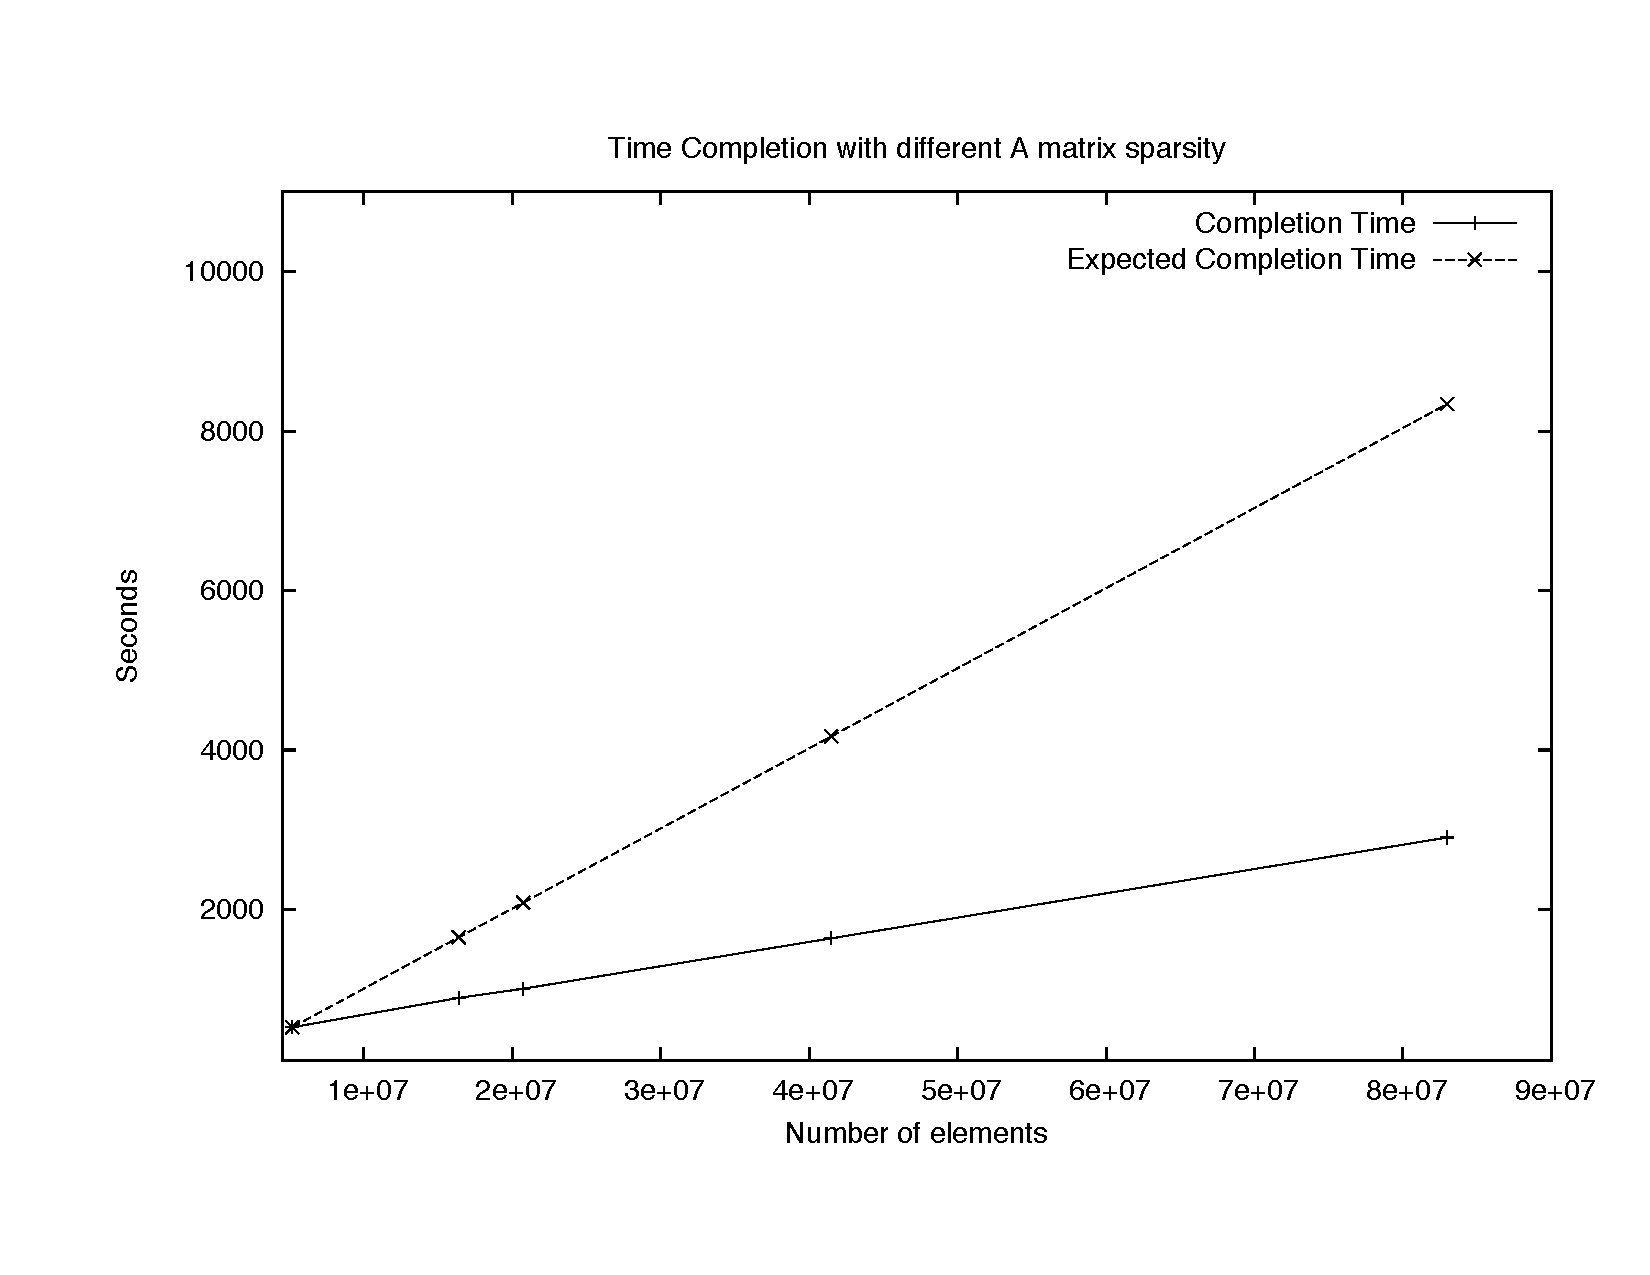
\includegraphics[scale=0.48]{HadoopTest/PsFiles/DeltaVar.pdf}}
	}
	\caption{Time Completion with different A matrix sparsity} 
        \label{DeltaVar}
\end{figure}

\begin{figure}[th]
	\centerline{
		\mbox{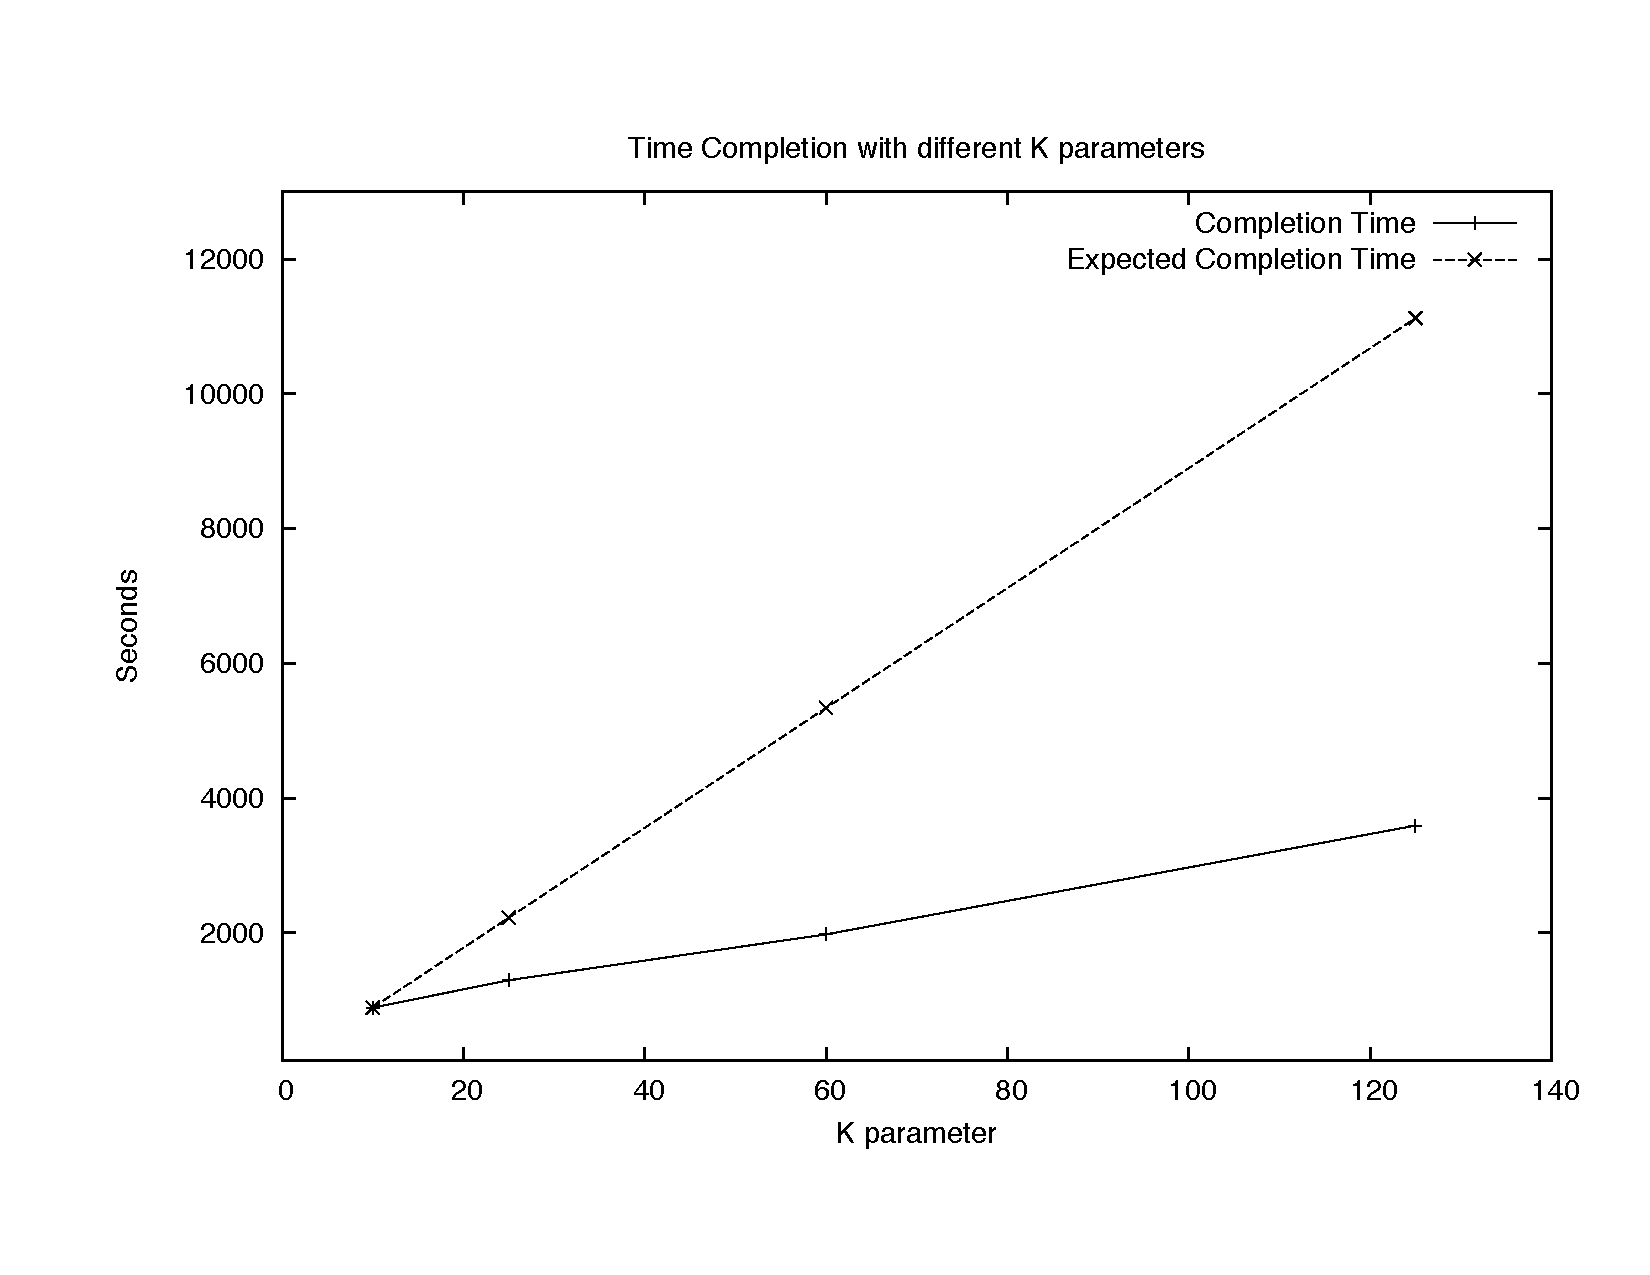
\includegraphics[scale=0.48]{HadoopTest/PsFiles/kVar.pdf}}
	}
	\caption{Time Completion with different K parameters} 
        \label{kVar}
\end{figure}


As we can see from both graphs, the behaviour of the test show a sub-linear dependencies from the size of the input data. \\

The second set of tests examines the behavior of the implementation when the parallel degree of the computation vary in the range between 1 and 21. 
The results of the test are reported in the figure \ref{NTime}  and \ref{NScal}. 
The first graph shows completion time while the second one on the scalability.

\begin{figure}[th]
	\centerline{
		\mbox{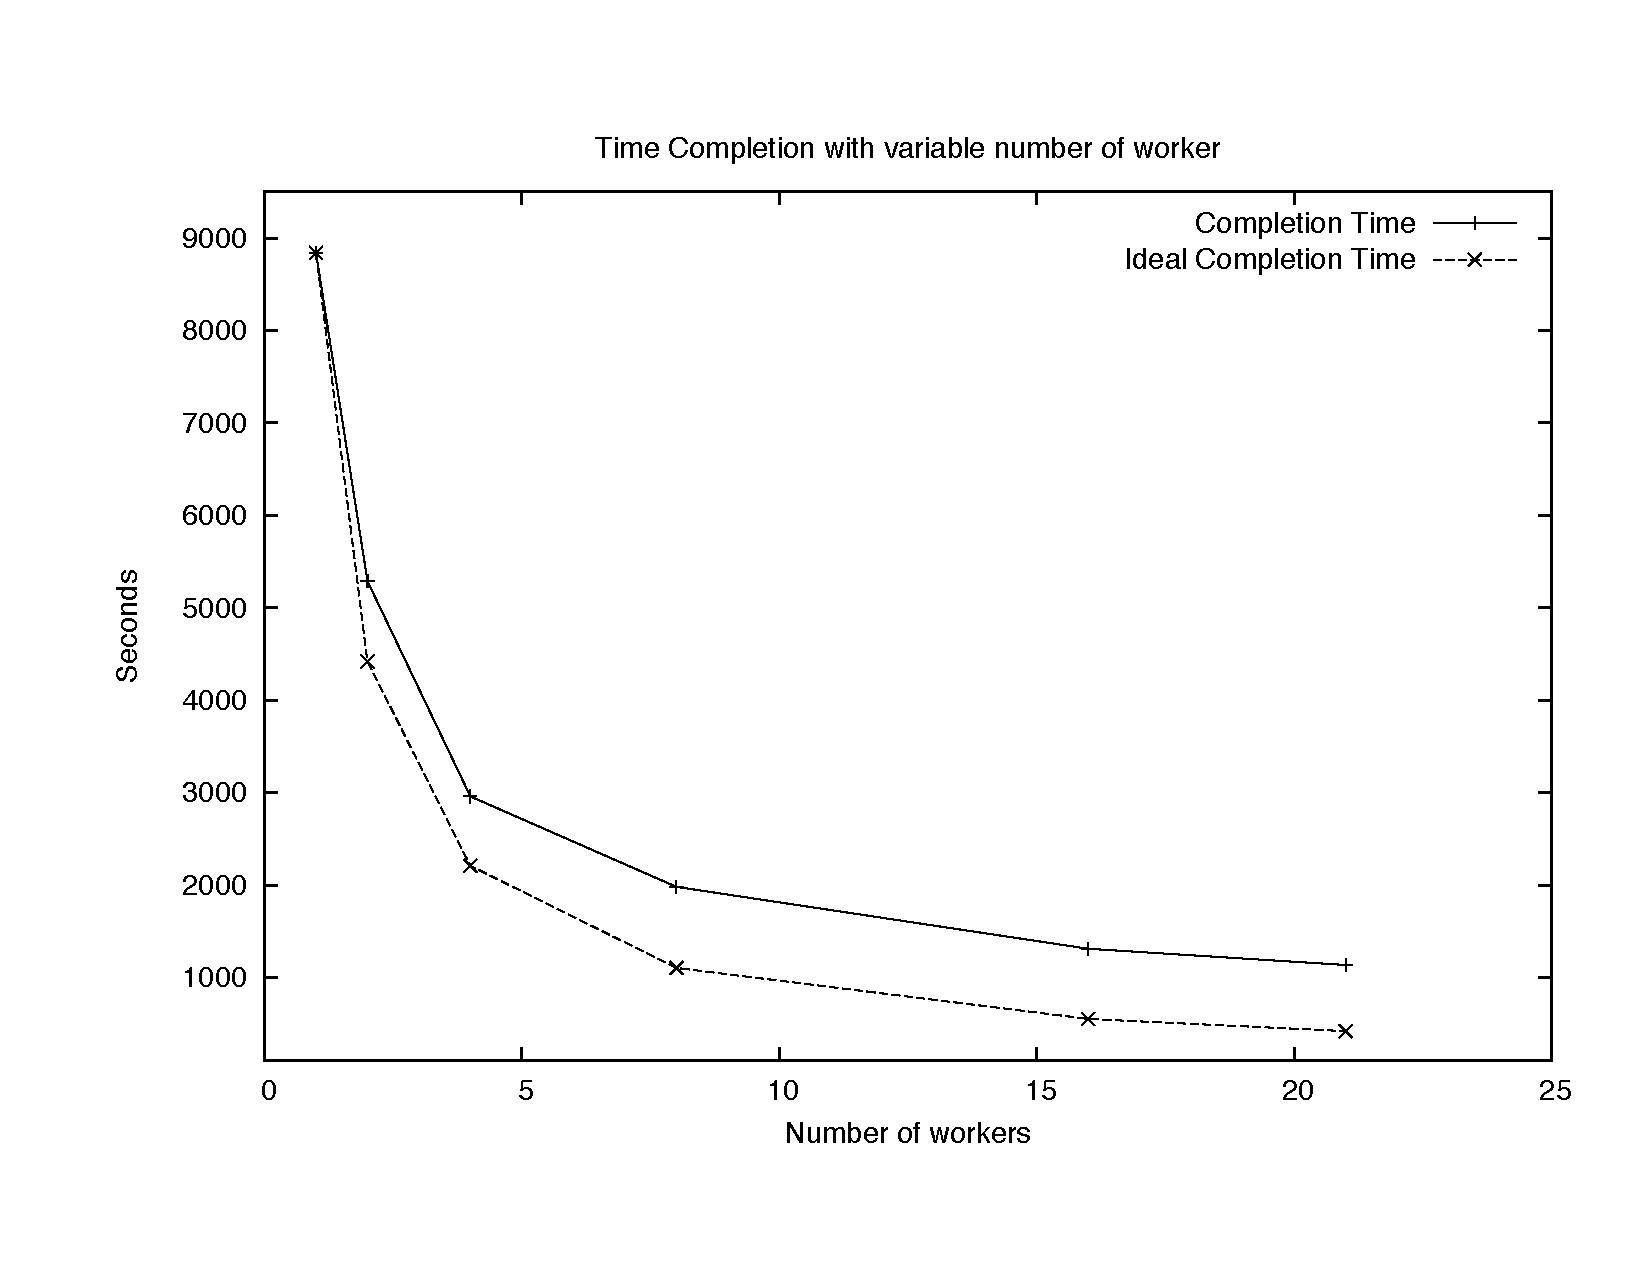
\includegraphics[scale=0.48]{HadoopTest/PsFiles/NTime.pdf}}
	}
	\caption{Completion time with respect of the number of workers.} 
        \label{NTime}
\end{figure}

\begin{figure}[th]
	\centerline{
		\mbox{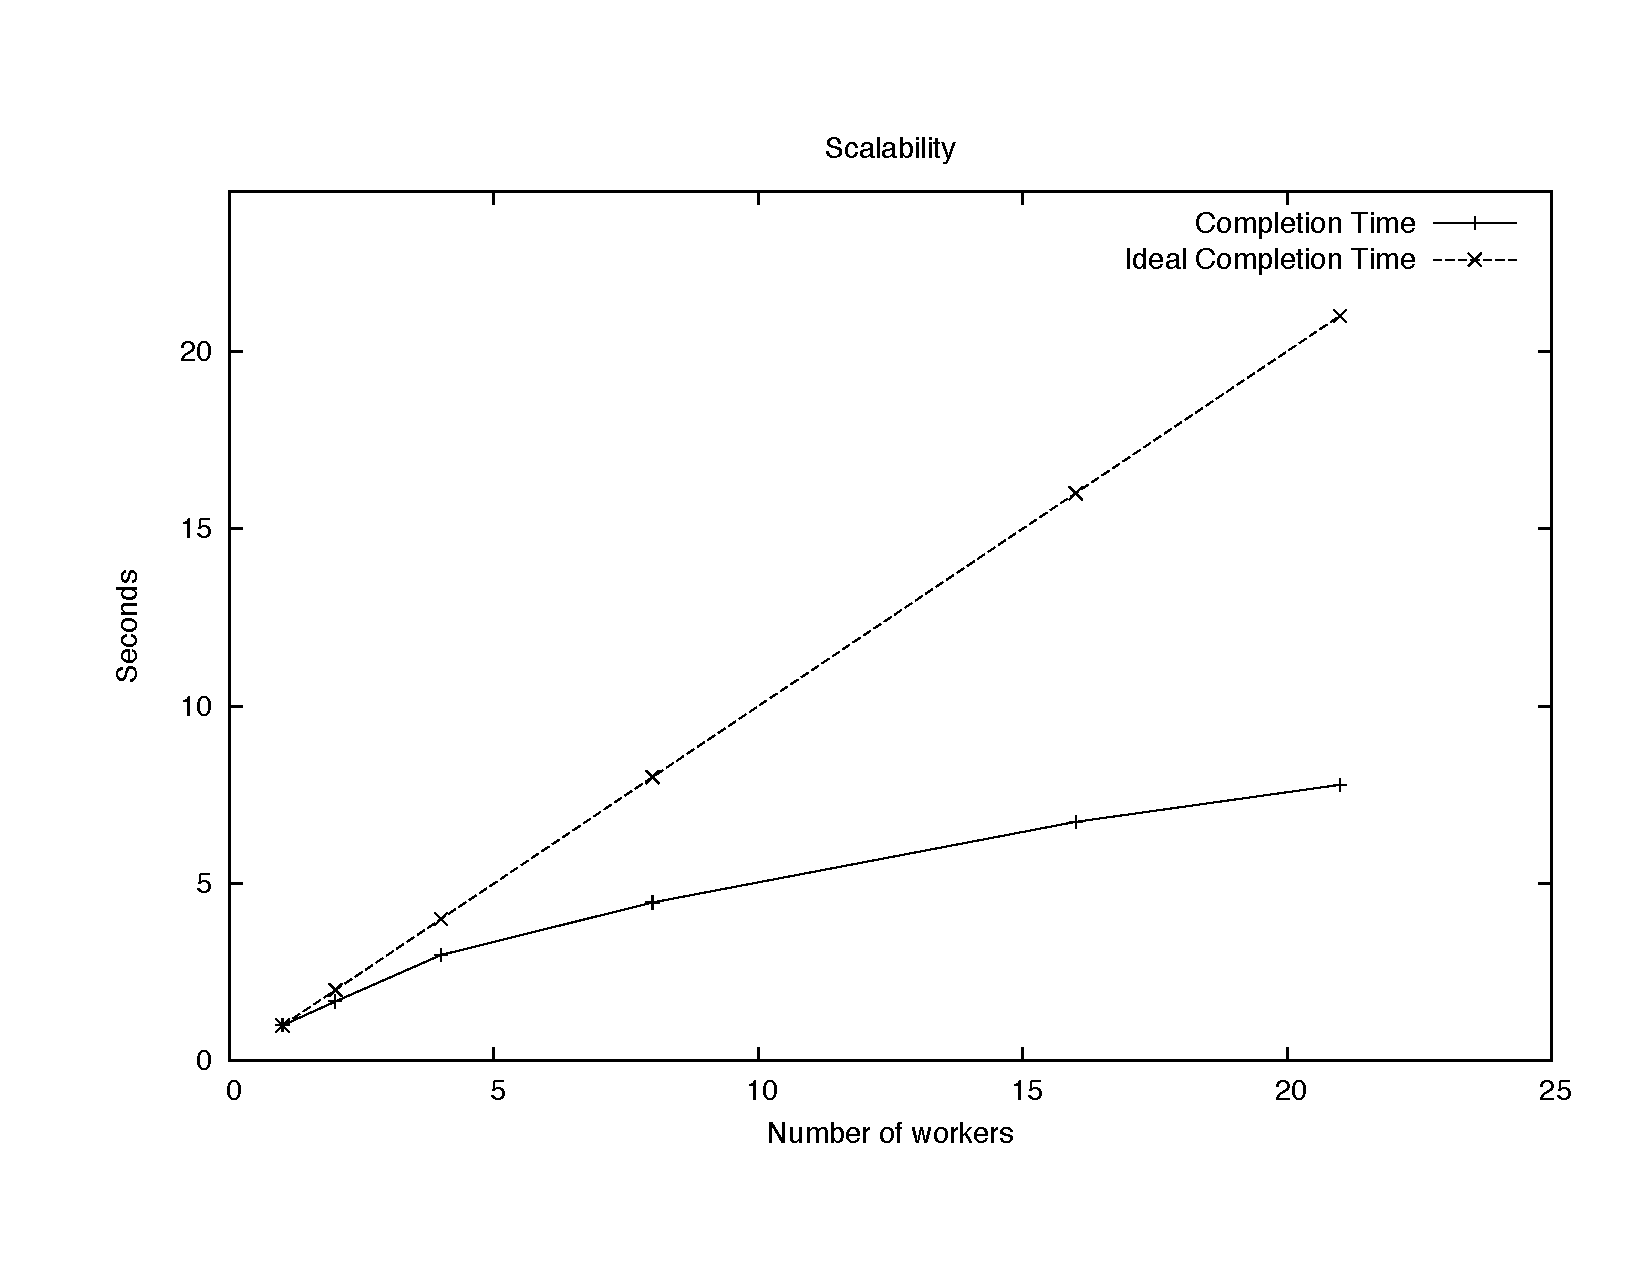
\includegraphics[scale=0.48]{HadoopTest/PsFiles/NScal.pdf}}
	}
	\caption{Scalability of the Application} 
        \label{NScal}
\end{figure}

As we can see from Figure \ref{NScal}, the algorithm does not have ideal scalability in Hadoop.
By analyzing the different phases (Table \ref{tab:differentPhases}) we can see that Phase 3 have limited scalability while phase 4 and 5 have no scalability at all.
\begin{table}[h!]
\begin{center}
\begin{tabular}{ | l || c | c | c | c |  c | c | }

  \hline      
  Phase & 1 & 2 & 4 & 8 &16 & 21 \\
  \hline      
  Phase 1 & 2242 	& 1492 & 797 	& 469 	& 320 	& 304\\
  Phase 2 & 1678 	& 885 	& 478	& 217 	& 191 	& 148\\
  Phase 3 & 92 		& 66 	& 48 	& 36 	& 33 	& 30\\ 
  Phase 4 & 23 		& 19 	& 21 	& 20 	& 20 	& 20\\
  Phase 5 & 66 		& 50 	& 55 	& 55 	& 54 	& 55\\
  \hline  


\end{tabular} 
  \end{center}
  \caption{Completion time of the five Phases with different parallelism degree.}
    \label{tab:differentPhases}
\end{table}
This might sound strange as phase 3, 4 and 5 are phases which are embarrassingly parallel.
However, their computational grain is very small.
Phase 3 performs a matrix multiplication of the narrow matrix W (for matrix H update) with itself; an operation of much smaller grain compared to the matrix vector multiplication performed in Phase 1 and 2. 
Similarly, phase 4 and 5 performs operations on a small set of data.
In fact, phase 1 and 2 dominate in the completion time; phase 3, 4 and 5 combined contribute for less than 20\%.
Consider that Hadoop is not suitable to perform computations of small grain.
As an example, in phase 5, (in which point-wise multiplication and division are performed on narrow matrices X,Y and H)  the shuffle phase takes most of the completion time (Table \ref{tab:Phase 5}). 
Moreover, the amount of time taken by the shuffle phase is almost unaffected by the variation of parallelism degree while the reduce phase (where multiplication is performed), although of very small grain, shows almost ideal scalability.
 
\begin{table}[h!]
\begin{center}
\begin{tabular}{ | l || c | c | c | c |  c | c | }

  \hline      
   						& 1 		& 2 		& 4 		& 8 		&16 		& 21 \\
  \hline      \hline
  Map Avg 		& 19 	& 14 	& 11 	& 9 		& 6 		& 9   \\
  Map Worst 		& 24 	& 22 	& 15		& 14 	& 9 		& 16  	\\
  \hline
  Shuffle Avg 	& 51 	& 37 	& 34 	& 33 	& 29 	& 30   \\ 
  Shuffle Worst 	& 53 	& 40 	& 37 	& 37 	& 32 	& 34   \\
  \hline
  Reduce Avg	& 16 	& 10 	& 6 		& 4 		& 3 		& 3     \\
  Reduce Worst	& 17 	& 11 	& 8 		& 5 		& 4 		& 5     \\
  \hline  
  Compl. Time &	99	&	74	&	66	&	63	&	56	&	59	\\
  \hline


\end{tabular} 
  \end{center}
  \caption{Completion time Phase 5 with respect to different parallelism degree.}
    \label{tab:Phase 5}
\end{table}





%\begin{center}
%\begin{tabular}{ | l || c | c | c | c |  c | c | }
%  \hline      
%  Phase & 1 & 2 & 4 & 8 &16 & 21 \\
%  \hline      
%  Phase 1 & 0,512 & 0,557 & 0,542 & 0,476 & 0,494 & 0,510\\
%  Phase 2 & 0,446 & 0,390 & 0,374 & 0,356 & 0,341 & 0,300\\
%  Phase 3 & 0,015 & 0,019 & 0,026 & 0,043 & 0,047 & 0,051\\ 
%  Phase 4 & 0,006 & 0,009 & 0,015 & 0,028 & 0,030 & 0,036\\
%  Phase 5 & 0,016 & 0,023 & 0,041 & 0,095 & 0,086 & 0,101\\
%  \hline  
%\end{tabular}
%\end{center}

Furthermore, we performed some additional tests in order to verify some of the assumptions that guided our implementation design. 
The first one regards Sequence Files.
We already explained in Section \ref{sec:implementation} why we used Sequence Files. 
Table \ref{tab:textvsSeq} show the completion time in the case that data is encoded as binary (Sequence Files) or Text. 
We can observe that we were correct and keeping data encoded it is beneficial for the application performance, especially for the phase 1 and 2.

\begin{table}
\begin{center}
\begin{tabular}{ | l || c | c | }
  \hline      
  & Text & Sequence \\
  \hline      
  Phase 1 & 475 & 264 \\
  Phase 2 & 333 & 105 \\
  Phase 3 & 66 & 42 \\ 
  Phase 4 & 18 & 15 \\
  Phase 5 & 36 & 35 \\
  \hline  
\end{tabular}
\end{center}
\label{tab:textvsSeq}
\caption{Comparison of completion time of the five phases of the application using Text and Sequence Files. }
\end{table}

Moreover we wanted to check how the combiner affects performances. 
The test is performed with A containing \numprint{16000000} elements, k is set to 25 and the parallel degree is 8.
Results are shown in Table \ref{comb_table}.

\begin{table}[h!]
\begin{center}

\begin{tabular}{ | l || c | c | }
  \hline      
  & \multicolumn{2}{|c|}{Record Number} \\
  & with Combiner & without Combiner \\
  \hline      
  H Phase 2 & 1896186 & 16406079 \\
  W Phase 2 & 678553 & 16406079 \\ 
  H Phase 3 & 14 & 105000 \\ 
  W Phase 3 & 14 & 20000 \\ 
 \hline  
  \hline      
  & \multicolumn{2}{|c|}{Completion Time} \\
  & with Combiner & without Combiner \\
  \hline      
  H Phase 2 & 217 & 426 \\
  W Phase 2 & 284 & 414 \\ 
  H Phase 3 & 36 & 136 \\ 
  W Phase 3 & 31 & 57 \\ 
 \hline  
\end{tabular}

\end{center}
\caption{Comparison of completion time and number of records processed for phases 3 and 4, with and without a combiner.}
\label{comb_table}
\end{table}














